\documentclass[a4paper, 12pt]{article}%тип документа

%%%Библиотеки
	%\usepackage[warn]{mathtext}	
	\usepackage[T2A]{fontenc} % кодировка
	\usepackage[utf8]{inputenc} % кодировка исходного текста
	\usepackage[english,russian]{babel} % локализация и переносы
	\usepackage{caption}
	\usepackage{listings}
	\usepackage{amsmath,amsfonts,amssymb,amsthm,mathtools}
	\usepackage{wasysym}
	\usepackage{graphicx}%Вставка картинок правильная
	\usepackage{float}%"Плавающие" картинки
	\usepackage{wrapfig}%Обтекание фигур (таблиц, картинок и прочего)
	\usepackage{fancyhdr} %загрузим пакет
	\usepackage{lscape}
	\usepackage{xcolor}
	\usepackage[normalem]{ulem}
	\usepackage{hyperref}

%%%Конец библиотек




%%%Настройка ссылок
	\hypersetup
	{
		colorlinks=true,
		linkcolor=blue,
		filecolor=magenta,
		urlcolor=blue
	}
%%%Конец настройки ссылок


%%%Настройка колонтитулы
	\pagestyle{fancy}
	\fancyhead{}
	\fancyhead[L]{Микроконтроллеры}
	\fancyhead[R]{ФРКТ, 2 курс}
	\fancyfoot[C]{\thepage}
%%%конец настройки колонтитулы



							\begin{document}
						%%%%Начало документа%%%%


%%%Начало титульника
\begin{titlepage}

	\newpage
	\begin{center}
		\normalsize Московский физико-технический институт \\(госудраственный 			университет)
	\end{center}

	\vspace{6em}

	\begin{center}
		\Large Введение в микроконтроллеры\\
	\end{center}

	\vspace{1em}

	\begin{center}
		\large \textbf{Светомузыка}
	\end{center}

	\vspace{2em}

	\begin{center}
		\large Рената Миндиярова Вилевна \\
			Ханин Александр Сергеевич \\
			Талашкевич Даниил Александрович \\
				
				
	\end{center}

	\vspace{\fill}

	\begin{center}
	Долгопрудный \\2022
	\end{center}
	
\end{titlepage}
%%%Конец Титульника



%%%Настройка оглавления и нумерации страниц
	\thispagestyle{empty}
	\newpage
	\tableofcontents
	\newpage
	\setcounter{page}{1}
%%%Настройка оглавления и нумерации страниц


					%%%%%%Начало работы с текстом%%%%%%
					
\section{Мотивация проекта}

Мотивацией выбора данного проекта была цель создать красивую и пригодную в быту установку, а так же научиться работать с адресной светодиодной лентой WS2812B, используя плату Arduino.


\section{What's inside?}

Светодиодная лента WS2812B реагирует на музыку, подключенную через разъем AUX 3,5 мм. Мы подключили 2 светодиодные ленты (WS2812B) и добавили возможность изменять эффекты путем нажатием кнопки.


Еще один важный этап : так как нашей $Arduino$ нужна библиотека $FAST LED$ и $NEOPIXEL$ для работы с $WS2812B$.

Поэтому мы загрузили библиотеки $FAST LED$ с $Github$ (ссылка в описании).

Аналогично загружаем библиотеку $NEOPIXEL$. 

Входной сигнал подается на аналоговые входы 4 и 5. Резистор на входе ленты необходим для ослабления "резких"импульсов, которые могут повредить первый светодиод.

\begin{figure}[!h]
\begin{center}
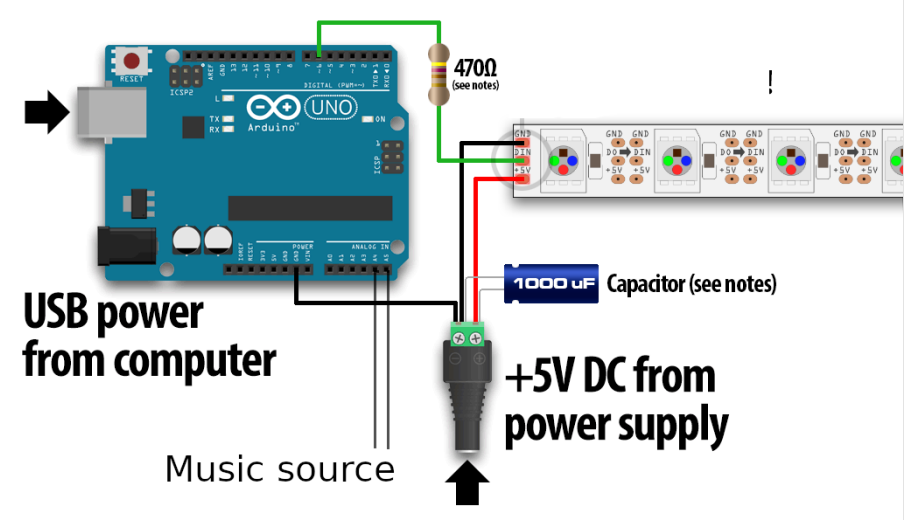
\includegraphics[scale=0.5]{pictures/scheme.png}
\end{center}
\end{figure}

Все исходники кода можно найти по ссылке в конце отчета.

\section{Сборочная составляющая}

Для того, чтобы проект приобрел человеческий вид была проделана следующая работа: за основу была взята коробка, кнопка переключения режимов была выведена наружу, светодиодные ленты были помещены в плафоны, все соединения спаены и надежно закреплены.


\begin{figure}[!h]
\begin{center}
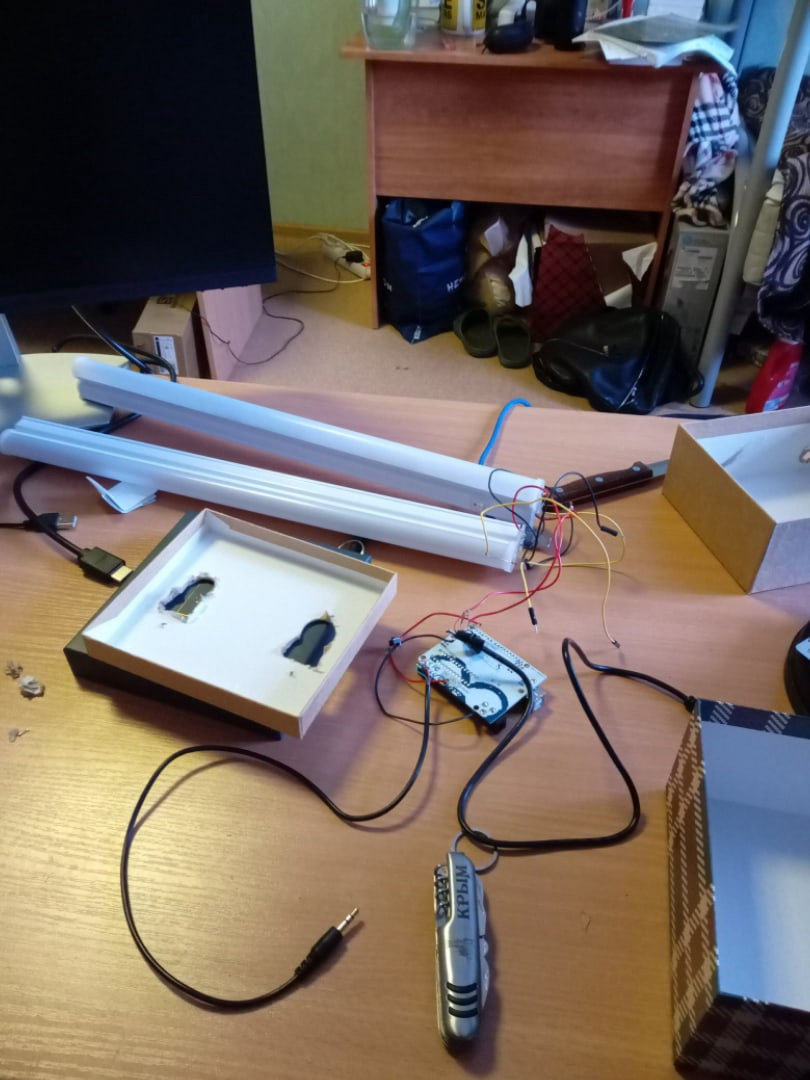
\includegraphics[scale=0.4]{pictures/work1.png}
\end{center}
\end{figure}

\section{Красивые картинки}



\section{Литература}


\begin{enumerate}

\item $«https://github.com/adafruit/Adafruit\_NeoPixel»$  (библиотеки).

\item $https://github.com/Hollbrok/light-music$ (исходники всего кода).

\end{enumerate}	

\end{document}
